\documentclass[letterpaper,12pt]{article}
\usepackage[letterpaper, portrait, margin=0.5in]{geometry}
\usepackage{graphicx}
\usepackage[utf8]{inputenc}
\usepackage[english]{babel}
\usepackage{fancyhdr}
\usepackage{multicol}
\graphicspath{{images/}}
\usepackage[export]{adjustbox}


\begin{document}
\noindent No escriba su nombre debajo de esta línea. \\
\noindent \hrule
\begin{center}
{\Large \textbf{\underline{Eventos y Secuencia}}}
\end{center}
Nombre de Usuario de Scratch: \rule{4cm}{0.4pt}

\noindent \dotfill \\

\noindent Los guiónes a continuacion pertenecen a un objeto llamado Gato: \\

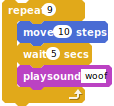
\includegraphics[scale=.55]{q1_script0.png} \hspace{.5cm}
\includegraphics[scale=.5]{q1_script1.png} \hspace{.5cm}
\includegraphics[scale=.5]{q1_script2.png} \hspace{.5cm}
\includegraphics[scale=.5]{q1_script3.png} \hspace{.5cm} \\

\noindent 1. \textbf{Circula}: ¿Qué debes hacer para que el Gato diga “Hola!”?
\renewcommand{\theenumi}{\Alph{enumi}}
\begin{enumerate}
\item Presiona la barra espaciadora
\item Haz clic en la bandera verde
\item Presiona la flecha hacia abajo
\item Haz clic en el objecto
\end{enumerate}

\noindent \dotfill \\

\noindent 2. \textbf{Circula} el bloque de Decir que se ejecutará al ultimo.  \\
\begin{center}
\includegraphics[scale=.5]{q2_script0.png}
\end{center}

\noindent \dotfill \\

\noindent 3. Los guiónes a continuacion pertenecen a un objeto. \textbf{Circula \underline{todos}} los guiones que se ejecutan al hacer clic en el objeto. \\

\includegraphics[scale=.5,valign=t]{q3_script0.png} \hspace{.1cm}
\includegraphics[scale=.5,valign=t]{q3_script1.png} \hspace{.1cm}
\includegraphics[scale=.5,valign=t]{q3_script2.png} \hspace{.1cm}
\includegraphics[scale=.45,valign=t]{q3_script3.png} \hspace{.1cm}


\newpage
\noindent  Cuando haces clic en la Bandera Verde, el escenario se ve así:
\begin{center}
\includegraphics[scale=.5]{q4_stage.png}
\end{center}

\noindent 4a. \textbf{Circula} el guión que corrió para la mariposa. \\ \\
\includegraphics[scale=.5,valign=t]{q4_script0.png} \hspace{.5cm}
\includegraphics[scale=.5,valign=t]{q4_script1.png} \hspace{.5cm}
\includegraphics[scale=.7,valign=t]{q4_script2.png} \hspace{.5cm}
\includegraphics[scale=.7,valign=t]{q4_script3.png} \hspace{.5cm}
\vspace{1cm}


\noindent 4b. \textbf{Circula} el guión que corrió para el perro. \\ \\
\includegraphics[scale=.5,valign=t]{q4_script0.png} \hspace{.5cm}
\includegraphics[scale=.5,valign=t]{q4_script1.png} \hspace{.5cm}
\includegraphics[scale=.7,valign=t]{q4_script2.png} \hspace{.5cm}
\includegraphics[scale=.7,valign=t]{q4_script3.png} \hspace{.5cm}
\vspace{.5cm}

\noindent \dotfill

\noindent Compara los dos guiónes a continuacion
\begin{center}
\includegraphics[scale=.5,valign=t]{q5_script0.png} \hspace{0.5in}
\includegraphics[scale=.5,valign=t]{q5_script1.png}
\end{center}

\noindent 5. \textbf{Circula} lo que es verdad:
\renewcommand{\theenumi}{\Alph{enumi}}
\begin{enumerate}
\item Hacen cosas diferentes. 
\item Hacen las mismas acciones en un orden diferente.
\item No hay diferencia.
\end{enumerate}
\noindent \dotfill \\

\newpage

\noindent Para la pregunta 6, por favor llene los espacios en blanco a continuación. \\ \\
\noindent 6. ¿Qué hará el objeto cuando se haga clic en la bandera verde?
\begin{center}
\includegraphics[scale=.5]{q6_script0.png}
\end{center}

\noindent Primero, \hrulefill . \\ \\
Siguiente, \hrulefill . \\ \\
Último, \hrulefill . \\ \\

\noindent \dotfill \\
Las preguntas 7a y 7b preguntan sobre el guión siguiente:
\begin{center}
\includegraphics[scale=.55]{q7_script0.png}
\end{center}

\noindent 7a. ¿Qué haces para que el guión se ejecute?
\renewcommand{\theenumi}{\Alph{enumi}}
\begin{enumerate}
\item Haz clic en la bandera verde
\item Haz clic en el sprite
\item Presiona la barra espaciadora\\
\end{enumerate}

\noindent 7b. ¿Qué hace el objeto cuando se ejecuta el guión? \\

\noindent Primero, \hrulefill . \\ \\
Siguiente, \hrulefill . \\ \\
Último, \hrulefill . \\



\end{document}